\documentclass{article}
\usepackage[utf8]{inputenc}

\title{Picture for scale params calculations}
\author{nagorny.denis }
\date{July 2020}

\usepackage{natbib}
\usepackage{graphicx}
\usepackage{tikz}

\begin{document}

\maketitle

\section{Introduction}
Lets create mapping between latency values into weight values

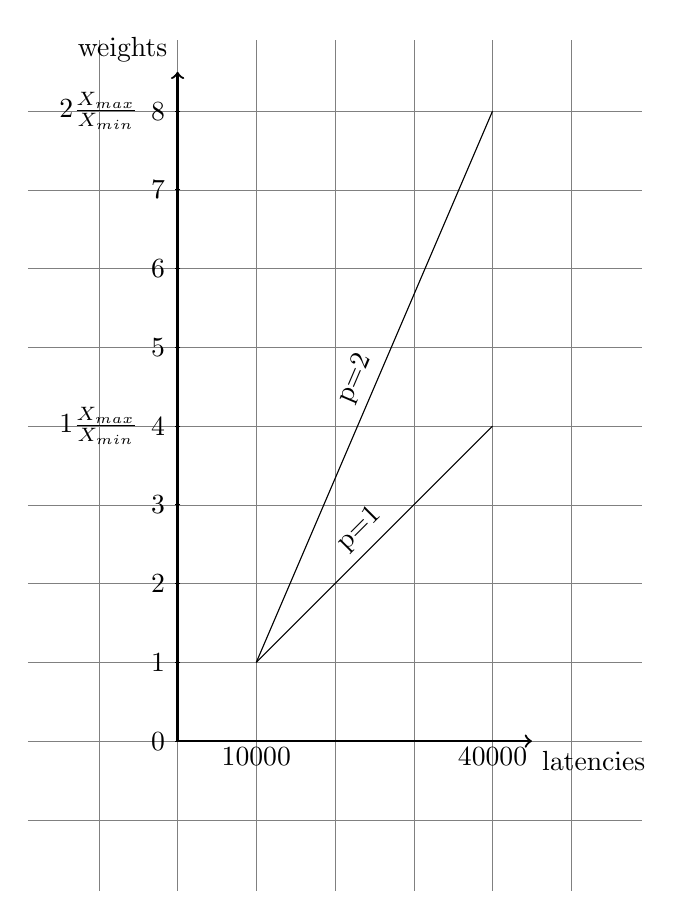
\begin{tikzpicture}
\draw[step=1cm,gray,very thin] (-1.9,-1.9) grid (5.9,8.9);
\draw[thick,->] (0,0) -- (4.5,0) node[anchor=north west] {latencies};
\draw[thick,->] (0,0) -- (0,8.5) node[anchor=south east] {weights};
\draw (1 cm,1pt) node[anchor=north] {10000};
\draw (4 cm,1pt) node[anchor=north] {40000};
\draw (1 cm, 1cm) -- (4 cm, 4cm) node[midway, sloped, above] {p=1};
\draw (1 cm, 1cm) -- (4 cm, 8cm)  node[midway, sloped, above] {p=2};
\draw (-1 cm, 4cm) node {$1\frac{X_{max}}{X_{min}}$};
\draw (-1 cm, 8cm) node {$2\frac{X_{max}}{X_{min}}$};
\foreach \y in {0,1,2,3,4,5,6,7,8}
    \draw (1pt,\y cm) -- (-1pt,\y cm) node[anchor=east] {$\y$};
\end{tikzpicture}


\end{document}

